\documentclass[a4paper]{report}

\usepackage{natbib}
\bibpunct{[}{]}{,}{a}{}{;}
\usepackage{fancyheadings}
\usepackage{iamdip}
\usepackage[pdftex]{graphicx}
\usepackage{caption}
\usepackage{subcaption}
\usepackage{amsmath}
\usepackage{amsthm}
\usepackage{amssymb}
\usepackage{amsfonts}
\usepackage{url}
\usepackage{hyperref}
\usepackage{array}

\usepackage{pdfpages}

\usepackage{listings}
\usepackage{xcolor}

\usepackage{pdflscape}
\usepackage{afterpage}

\definecolor{dkgreen}{rgb}{0,0.6,0}
\definecolor{gray}{rgb}{0.5,0.5,0.5}
\definecolor{mauve}{rgb}{0.58,0,0.82}

\lstdefinestyle{inline}
{
numbers=left,
xleftmargin=1cm,
belowskip=3mm,
moredelim=**[is][\color{red}]{\$}{\$},
moredelim=**[is][\color{green}]{^}{^}
}

\lstdefinestyle{table}
{
numbers=none,
xleftmargin=0mm,
belowskip=0mm,
moredelim=**[is][\color{red}]{\$}{\$},
moredelim=**[is][\color{green}]{^}{^}
}

\lstset{frame=none,
  language=Java,
  aboveskip=3mm,
  showstringspaces=false,
  columns=flexible,
  basicstyle={\small\ttfamily},
  numberstyle=\tiny\color{gray},
  keywordstyle=\color{blue},
  commentstyle=\color{dkgreen},
  stringstyle=\color{mauve},
  breaklines=true,
  breakatwhitespace=true,
  tabsize=3,
  style=table
}


\headrulewidth 0.5pt \addtolength{\headheight}{5pt}

\lhead[\fancyplain{}{\rm\thepage}]{\fancyplain{}{\rightmark}}
\rhead[\fancyplain{}{\leftmark}]{\fancyplain{}{\rm\thepage}}
\cfoot{}

% \graphicspath{{../Figures/}}
\graphicspath{ {images/} }

\DeclareMathOperator{\score}{score}

\begin{document}

\pagestyle{fancyplain} \thispagestyle{empty}

\title{TITLE}
\author{Sven Kellenberger}
\betreuer{Prof. Dr. Paolo Favaro}
\ort{Bern}
\datum{01.08.2018}

\pagenumbering{roman} \setcounter{page}{1}
\maketitle

\newpage
\thispagestyle{empty}
\vspace{8cm}
\noindent
{\centerline {\bf \large Abstract}}
\vspace{1cm}


\noindent

Lorem ipsum dolor sit amet, consetetur sadipscing elitr, sed diam nonumy eirmod tempor invidunt ut labore et dolore magna aliquyam erat, sed diam voluptua. At vero eos et accusam et justo duo dolores et ea rebum. Stet clita kasd gubergren, no sea takimata sanctus est Lorem ipsum dolor sit amet. Lorem ipsum dolor sit amet, consetetur sadipscing elitr, sed diam nonumy eirmod tempor invidunt ut labore et dolore magna aliquyam erat, sed diam voluptua. At vero eos et accusam et justo duo dolores et ea rebum. Stet clita kasd gubergren, no sea takimata sanctus est Lorem ipsum dolor sit amet. Lorem ipsum dolor sit amet, consetetur sadipscing elitr, sed diam nonumy eirmod tempor invidunt ut labore et dolore magna aliquyam erat, sed diam voluptua. At vero eos et accusam et justo duo dolores et ea rebum. Stet clita kasd gubergren, no sea takimata sanctus est Lorem ipsum dolor sit amet.

Duis autem vel eum iriure dolor in hendrerit in vulputate velit esse molestie consequat, vel illum dolore eu feugiat nulla facilisis at vero eros et accumsan et iusto odio dignissim qui blandit praesent luptatum zzril delenit augue duis dolore te feugait nulla facilisi. Lorem ipsum dolor sit amet, consectetuer adipiscing elit, sed diam nonummy nibh euismod tincidunt ut laoreet dolore magna aliquam erat volutpat.

Ut wisi enim ad minim veniam, quis nostrud exerci tation ullamcorper suscipit lobortis nisl ut aliquip ex ea commodo consequat. Duis autem vel eum iriure dolor in hendrerit in vulputate velit esse molestie consequat, vel illum dolore eu feugiat nulla facilisis at vero eros et accumsan et iusto odio dignissim qui blandit praesent luptatum zzril delenit augue duis dolore te feugait nulla facilisi.

Nam liber tempor cum soluta nobis eleifend option congue nihil imperdiet doming id quod mazim placerat facer


\pagenumbering{roman} \setcounter{page}{1}
\tableofcontents
\newpage{\pagestyle{empty} \cleardoublepage}

\pagenumbering{arabic} \setcounter{page}{1}
\pagestyle{fancy}

\chapter{Introduction}
\section{Motivation}
Automatic text correction is a ubiquitous technology in our today world. Every smartphone, every word processing software, every browser provides some form of spelling error detection and correction for text input. These systems usually rely on a dictionary of correct words \cite{dictionary_correction, digram_correction} or some machine learning algorithm \cite{seq2seq_on_text_correction} to find errors and possible corrections.

Source code is very sensitive to errors of all kinds and therefore this functionality is also desirable for code editors. The syntax of a programming language is strictly defined which enables integrated development environments (IDEs) to detect syntax errors before the program is even run. Of course the possibilities of an IDE are limited by the properties of the programming language, e.g. is it strongly typed or weakly typed. However, the error detection in source code is mostly limited to syntax errors, while semantic and logical errors show only at runtime or sometimes go completely unnoticed. These kinds of errors are also the hardest ones to fix. In a strongly typed language like Java, a lot of possible errors in naming and accessing attributes can be eliminated, because each variable has to be initiated before it is used and the type of the variables is known at all times and therefore also their available attributes and methods. In weakly typed languages like Ruby however, one can not determine what type of object a variable holds before runtime. This creates additional sources of runtime errors.

While syntax errors can be detected by a suitable algorithm, traditional algorithms can only hope to help prevent semantic and logical errors. This is where machine learning algorithms could step in. In the past years, deep neural networks have proven to be very effective in learning generalised concepts and applying them to single cases. For example in \cite{style_transfer} a network is trained to transfer the style of a painting to a video sequence. That's why it should also be possible to train a network to recognize and correct certain logic errors in source code.

The aim of this project is it to train a character based sequence-to-sequence model on the task of source code correction. The implementation of the model is based on the neural machine translation (NMT) model provided by Tensorflow \cite{seq2seq_tutorial}. As a dataset the Java Github Corpus \cite{java_dataset} is used as a source of correct data. This data is then perturbed as random syntax, semantic and logic errors are added. The performance of different model architectures is then evaluated for the introduced errors.

\section{Outline}

This thesis is divided into five chapters, including this introduction. In the second chapter an overview of the prior work on the task of spelling checking and correction is given and also some work on error detection and correction in source code. Furthermore a short introduction to the machine learning techniques and architectures used in this thesis is given. The third chapter provides a description of the used model, the training procedure and the dataset construction. In chapter four the experiments are explained and the optained results analysed. Chapter five provides the conclusion and suggestions for future work.

\newpage{\pagestyle{empty} \cleardoublepage}

\chapter{Background}
\section{Origins of Spelling Checkers and Correctors}

With the emergence of word processing programs and the following digitalization of text documents, spelling checkers and correctors have become a common helper in our everyday lives. However, the research on this topic has begun much earlier \cite{program_check_correction}.

The original motivation for a spelling checker was to find input errors in databases. For example, in \cite{data_correction} the authors aim to find incorrectly spelled names, dates and places in a genealogical database. This is done by computing the frequency of trigrams (three sequential characters) in the source text and based on that the probability of a character given some context, i.e. its adjacent characters. Erroneous words are found by looking at its trigrams. If a word consist of a number of unusual character combinations, it is probably spelled wrongly. However, it is easy to see that this method is not very useful for new, rare or foreign expressions like \texttt{doppelg\"{a}nger} and for typos with high probabilities of being correct. Furthermore the model is limited to the vocabulary used in the text.

These problems were solved by the introduction of dictionaries. A dictionary is a list of correctly spelled words which can optionally be extended by the user. For every word, the program checks if it is part of the dictionary. If it is, then it is spelled correctly, otherwise there is an error. This method was enhanced by the addition of direct user interaction. Instead of outputting a list of incorrect words, the program would show the user the words it assumed to be incorrectly spelled and then give the user some possible actions to chose from.

Spelling correction is another enhancement of these methods. In \cite{dictionary_correction} a dictionary is used to find incorrect words. It is assumed that these words contain only one of four types of errors: one character was wrong, one extra character was inserted, one character was missing or two adjacent characters were transposed. Under this assumption the dictionary is searched for possible corrections. In \cite{digram_correction} the author uses a dictionary to find incorrect words as well. For the found words he uses digrams (similar to the trigrams mentioned above, just with two instead of three characters) to suggest corrections for incorrect words.

\begin{figure}
\centering
\begin{subfigure}[b]{.5\textwidth}
  \centering
  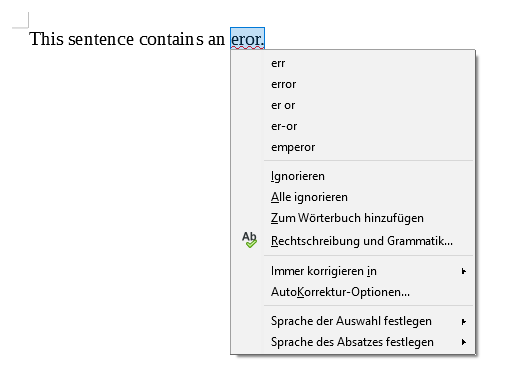
\includegraphics[width=\linewidth]{word_error}
  \caption{A subfigure}
  \label{fig:sub1}
\end{subfigure}%
\begin{subfigure}[b]{.5\textwidth}
  \centering
  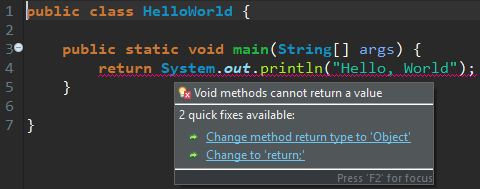
\includegraphics[width=\linewidth]{eclipse_error}
  \caption{A subfigure}
  \label{fig:sub2}
\end{subfigure}
\caption{A figure with two subfigures}
\label{fig:test}
\end{figure}

\subsection{Modern Research}

Of course the methods described so far do still not take the context of the text into account. For example if \texttt{know} is misspelled as \texttt{now}, no error is indicated even though it could be concluded from the context that a verb is expected in this place. This "context-awareness" has been the topic of a lot of recent research. In \cite{context_n_gram} n-grams are used to determine the most likely replacement for an error and in \cite{context_sensitive_spelling} the authors concentrate on finding and correcting small spelling errors that result in correct words and are therefore not detected by a traditional spelling checker (e.g. \texttt{to} for \texttt{too} or \texttt{there} for \texttt{their}). Other researchers concentrated on a particular set of errors like article \cite{article_correction} or preposition errors \cite{preposition_correction}.

However, even though these methods perform well on the errors they were designed for, a large amount of different classifiers is needed to catch every error. This is a costly and inflexible approach. Recent research often uses statistical machine translation methods or language models and n-grams to correct errors of multiple classes \cite{grammatical_error_task}. In \cite{seq2seq_on_text_correction} the authors train an encoder-decoder neural network with an attention mechanism which operates at the character level. \cite{seq2seq_keyboard} chose a similar approach applied to keyboard decoding on smartphones.

\section{Automatic Correction of Source Code}

Of course automatic error correction is also a useful helper for writing code. Because of the well-defined syntax of a programming language, syntactical errors are relatively easy to find using an algorithm. This functionality can help novice programmers to avoid typical beginner's errors like a missing semicolon at the end of the line. However, semantic and logical errors can usually not be detected this easily.

The correctability of a programming language depends in part on its properties. One important distinction is between strongly typed and weakly typed programming languages \cite{pl_typing}. In a strongly typed programming language, every variable has a fixed type and every method has a fixed return type. This enables an editor program to check if the expected and the actual type match before runtime. This error can then be flagged and shown to the user. In contrast, in a weakly typed programming language, variables don't have a fixed type. They can contain whatever value one assigns to them and similarly methods can take arguments of any type and also return values of any type. In this case, an error of an operation which gets an unexpected parameter type only shows at runtime. For example on the one hand, the type error in

\lstset{belowskip=3mm}
\begin{lstlisting}
public int increment(int a){
  return ++a;
}
int result = increment("a");
\end{lstlisting}

\noindent can be detected before runtime because Java is a strongly typed programming language. The type of the parameter \texttt{a} is defined as \texttt{int} and the method invocation with an argument of type \texttt{String} is clearly wrong. On the other hand the type error in

\lstset{language=Python}
\begin{lstlisting}
a = 10
print("The number ten: " + a)
\end{lstlisting}
\lstset{language=Java}
\lstset{belowskip=0mm}

shows only at runtime. Python is a weakly typed language and in general it can not be determined what type of value a variable holds before runtime. Only when the code is executed, the \texttt{+} operator looks at its arguments and throws an error if their types don't match.

\newpage{\pagestyle{empty} \cleardoublepage}

\chapter{Model and Training}
\section{Components}

\subsection{LSTM}

A recurrent neural network (RNN)\cite{rnn} is a special form of neural network that is used for sequential tasks. It works by having multiple copies of the network, one for each timestep. As the input proceeds in time, each network passes information to it's next instance as seen in  \textcolor{red}{INSERT FIGURE HERE}. For an input sequence \((\mathbf{x}_1, ..., \mathbf{x}_n)\) the RNN produces at each timestep \(t\) a hidden state vector \(\mathbf{h}_t\) as follows:

\begin{equation*}
  \mathbf{h}_t = \tanh \left(\mathbf{W} \begin{pmatrix} \mathbf{x}_t \\ \mathbf{h}_{t-1} \end{pmatrix} \right)
\end{equation*}

However, RNNs have proven to be hard to train, especially on long-range dependencies \cite{hochreiter_rnn}. In theory, they should be able to deal with these dependencies but either vanishing or exploding gradients usually prevent them from doing so. To solve this issue, Long Short-Term Memory networks (LSTMs) \cite{lstm} were proposed. In addition to \(\mathbf{h}_t\), LSTMs also pass a memory state vector \(\mathbf{c}_t\) to the next instance as can be seen in \textcolor{red}{INSERT FIGURE HERE}. The LSTM can choose at each timestep if it wants to read or forget information from the memory vector or write new information onto the vector. This is done by using explicit gating mechanisms:

\begin{align*}
  \mathbf{f}_t &= \sigma \left(\mathbf{W}_f \begin{pmatrix} \mathbf{x}_t \\ \mathbf{h}_{t-1} \end{pmatrix} \right) &
  \mathbf{i}_t &= \sigma \left(\mathbf{W}_i \begin{pmatrix} \mathbf{x}_t \\ \mathbf{h}_{t-1} \end{pmatrix} \right) \\
  \mathbf{o}_t &= \sigma \left(\mathbf{W}_o \begin{pmatrix} \mathbf{x}_t \\ \mathbf{h}_{t-1} \end{pmatrix} \right) &
  \mathbf{g}_t &= \tanh \left(\mathbf{W}_g \begin{pmatrix} \mathbf{x}_t \\ \mathbf{h}_{t-1} \end{pmatrix} \right)
\end{align*}

\noindent where \(\sigma\) is the sigmoid function. \(\mathbf{f}_t\), \(\mathbf{i}_t\) and \(\mathbf{o}_t\) can be thought of as binary gates that decide which information from \(\mathbf{c}_{t-1}\) should be deleted, which information of \(\mathbf{c}_{t-1}\) should be updated and which information from \(\mathbf{c}_t\) should be written to \(\mathbf{h}_t\).  Finally \(\mathbf{g}_t\) is a vector of possible values that (gated by \(\mathbf{i}_t\)) can be added to \(\mathbf{c}_{t-1}\) and because of the \(\tanh\) in the equation its values may range from \texttt{-1} to \texttt{1}. The state vectors are then updated as follows:

\begin{align*}
  \mathbf{c}_t &= \mathbf{f}_t \odot \mathbf{c}_{t-1} + \mathbf{i}_t \odot \mathbf{g}_t \\
  \mathbf{h}_t &= \mathbf{o}_t \odot \tanh(\mathbf{c}_t)
\end{align*}

Almost all remarkable results that are achieved today are achieved using either LSTMs or networks with a similar architecture like Gated Recurrent Units (GRUs) \cite{gru} because they are easier to train and excel at capturing long range dependencies.

\subsection{The Sequence-to-Sequence Model}

Traditional Deep Neural Networks (DNNs) process the whole input and then calculate some output, e.g. process an image and then classify it. This works well for problems where the input and the output are of a fixed dimension, however it is not suitable for problems where the input and the output are sequences of variable length. An example would be the input of a question and the network should produce an answer. We have seen that we can use LSTMs to process input sequences of variable length. However, in this case we want to process the whole input sequence and all the information that comes with it and only then start generating an output sequence. These problems are called sequence to sequence problems.

In \cite{seq2seq} the Sequence-to-Sequence Model is introduced as a solution to these problems. The model was applied to the task of Neural Machine Translation (NMT) and has since become the state of the art architecture in this field. The main concept can be seen in \textcolor{red}{FIGURE X}. First the whole input sequence is fed into the network and the output is ignored. Then we input an end-of-sequence token \texttt{<EOS>} which signals the network to start producing the output. From there on the produced output tokens are fed to the network until the an end-of-sequence token is generated, thus signaling the end of the sequence. To speed up training the expected output is fed back to the network and not the actual produced output.

This architecture is further improved by splitting the network into two separate LSTMs (\textcolor{red}{FIGURE}). The first network takes all the input and encodes it into a vector which is then used to initialize the second network. It is first fed a start token \texttt{<GO>} and then the generated output until the end of the sequence is reached.

The network usually operates at word level and uses some word embedding like word2vec \cite{word2vec}. This method has the advantage of giving the input words some meaning through the embedding instead of just inputting a meaningless encoding of the word. While this is very effective for translation tasks, there are some limitations to this method. These embeddings work on a fixed size vocabulary which means that out of vocabulary words (OOV) can't be handled. Also special character sequences like \texttt{:)} pose a problem.

\subsection{Attention-Mechanism}

Attention is a relatively new concept for neural networks. The idea is to allow the network to chose on which information to focus at any given moment. For example in \cite{visual_attention} attention is used on the task of high resolution image classification. These kind of networks often struggle with memory constraints and attention can help them to only load the significant part of the image into the memory.

Attention has subsequently been applied to NMT \cite{attention_luong,attention_bahdanau}. The vector into which the input is encoded in the Sequence-to-Sequence model has been identified as a bottleneck which cuts down performance because of its limited capacity. After all the vector is of fixed dimensionality and needs to encode information about the whole input sequence. Because of that attention is used as a mean for the decoder to peek at previous hidden states of the encoder. This is done via a context vector \(\tilde{\mathbf{c}}_t\) which is combined with the current hidden state of the decoder \(\mathbf{h}_t\). The resulting attentional hidden state \(\tilde{\mathbf{h}}_t\) is then used by the decoder to generate the next output.

\begin{equation*}
  \tilde{\mathbf{h}}_t = \tanh \left(\mathbf{W}_c \begin{pmatrix} \tilde{\mathbf{c}}_t \\ \mathbf{h}_{t} \end{pmatrix} \right)
\end{equation*}

For the derivation of the context vector \(\tilde{\mathbf{c}}_t\) all hidden states of the encoder \(\bar{\mathbf{h}}_s\) are considered. For this an alignment vector \(\mathbf{a}_t\), whose size equals the input sequence length, is calculated from the current decoder hidden state \(\mathbf{h}_t\) and the encoder hidden states \(\bar{\mathbf{h}}_s\). The values of \(a_t\) are then normalized using the \texttt{softmax} function.

\begin{equation*}
  a_t(s) = \frac
            {\exp(\score(\mathbf{h}_t, \bar{\mathbf{h}}_s))}
            {\sum_{s'} \exp(\score(\mathbf{h}_t, \bar{\mathbf{h}}_{s'}))}
\end{equation*}

Here, \(\score\) is a content-based function used to compare the decoder hidden state \(\mathbf{h}_t\) with each of the encoder hidden states \(\bar{\mathbf{h}}_s\). There are various possible choices for this function, for example:

\begin{equation*}
  \score(\mathbf{h}_t, \bar{\mathbf{h}}_s) =
  \begin{cases}
    \mathbf{h}_t^\intercal \mathbf{W}_a \bar{\mathbf{h}}_s \\
    \mathbf{v}_a^\intercal \tanh \left(\mathbf{W}_a \begin{pmatrix} \mathbf{h}_t \\ \bar{\mathbf{h}}_s \end{pmatrix} \right)
  \end{cases}
\end{equation*}

The context vector \(\mathbf{c}_t\) is then calculated as the weighted average over the encoder hidden states.

\begin{equation*}
  \mathbf{c}_t = \sum_{s'} a_t(s') \bar{\mathbf{h}}_{s'}
\end{equation*}

\section{Implementation}

\section{Dataset Construction}

\newpage{\pagestyle{empty} \cleardoublepage}

\chapter{Experiments and Results}
To get good results some experiments were conducted first to find the best possible architecture. After that, the obtained results were analyzed on in regard of the different corruption types.

\section{Experiments}

\subsection{Corruption Rate}

\begin{table}[t]
\begin{subtable}{\linewidth}\centering
{\begin{tabular}{ | r | r |r | r | r | r |r | }
  \hline
  & NC & MS & MB & VAR & RET & SL \\
  \hline
  \hline
  100\% & 60.0 & 64.0 & 48.2 & \textbf{37.3} & 54.3 & 26.7 \\
  \hline
  75\% & \textbf{70.4} & \textbf{71.8} & \textbf{51.3} & 34.4 & \textbf{55.1} & \textbf{42.6} \\
  \hline
  50\% & 62.0 & 61.2 & 43.7 & 25.0 & 47.4 & 26.1 \\
  \hline
  25\% & 67.9 & 65.6 & 41.6 & 19.6 & 50.3 & 33.3 \\
  \hline
\end{tabular}}
\caption{Performance of models with different corruption rates.}\label{corruption_rate_table}
\end{subtable}
\newline
\vspace*{5mm}
\newline
\begin{subtable}{\linewidth}\centering
{\begin{tabular}{ | m{3cm} | r | r | r | r | r | r | }
  \hline
  & NC & MS & MB & VAR & RET & SL \\
  \hline
  \hline
  with attention & \textbf{70.4} & \textbf{71.8} & \textbf{51.3} & \textbf{34.4} & \textbf{55.1} & \textbf{42.6} \\
  \hline
  without attention & 0.0 & 0.0 & 0.0 & 0.0 & 0.0 & 0.0 \\
  \hline
  without attention, input reversed & 0.0 & 0.0 & 0.0 & 0.0 & 0.0 & 0.0 \\
  \hline
\end{tabular}}
\caption{Performance of models with or without an attention mechanism.}\label{attention_mechanism_table}
\end{subtable}
\newline
\vspace*{5mm}
\newline
\begin{subtable}{\linewidth}\centering
{\begin{tabular}{ | l | r | r | r | r | r | r | }
  \hline
  & NC & MS & MB & VAR & RET & SL \\
  \hline
  \hline
  LSTM & \textbf{70.4} & \textbf{71.8} & \textbf{51.3} & \textbf{34.4} & \textbf{55.1} & \textbf{42.6} \\
  \hline
  GRU & 0.2 & 0.2 & 0.2 & 0.2 & 0.2 & 0.2 \\
  \hline
  vanilla RNN & 0.0 & 0.0 & 0.0 & 0.0 & 0.0 & 0.0 \\
  \hline
\end{tabular}}
\caption{Performance of different RNN types.}\label{rnn_type_table}
\end{subtable}
\caption{Evaluation of the performance of the models on the test set with different corruptions: uncorrupted (NC), missing semicolon (MS), missing bracket (MB), misspelled variable (VAR), wrong return type (RET) and line switch (SL).}
\end{table}

Because the source sequence and target sequence are almost the same and the errors are self-introduced, it is an interesting question what the optimal corruption rate for the input is. To test this the model was trained with four different corruption rates, 100\%, 75\%, 50\% and 25\%. The results can be seen in Table \ref{corruption_rate_table}.

For almost all corruptions the model trained with a corruption rate of 75\% posted the best result. The models with lower percentages didn't pick up on the errors as well while the model with the 100\% corruption rate didn't get as good an understanding of when the code is correct. In general, the model learned to correct all of the introduced errors. It performed especially well when inputting a sequence missing a single semicolon which is of course also the simplest task to solve. However, the model was also able to correct the other errors reasonably well. A missing bracket or an incorrect return type were corrected most of the time while the model had a little more trouble correcting a misspelled variable or realigning switched lines. A more detailed analysis of the different error types is given in Section \ref{error_analysis}.

What is also interesting to see is how well the model performed on uncorrupted sequences. Even the model with 100\% corruption rate, i.e. which never got an uncorrupted sequence as input, managed to not introduce any new errors into an uncorrupted sequence most of the time. This indicates that the model obtains some understanding of the input and how code works and only corrects where necessary.

Going forward all experiments were done with a corruption rate of 75\% and the error analysis was also done on the results of this model.

\subsection{Attention Mechanism}

\begin{figure}[p]
\centering
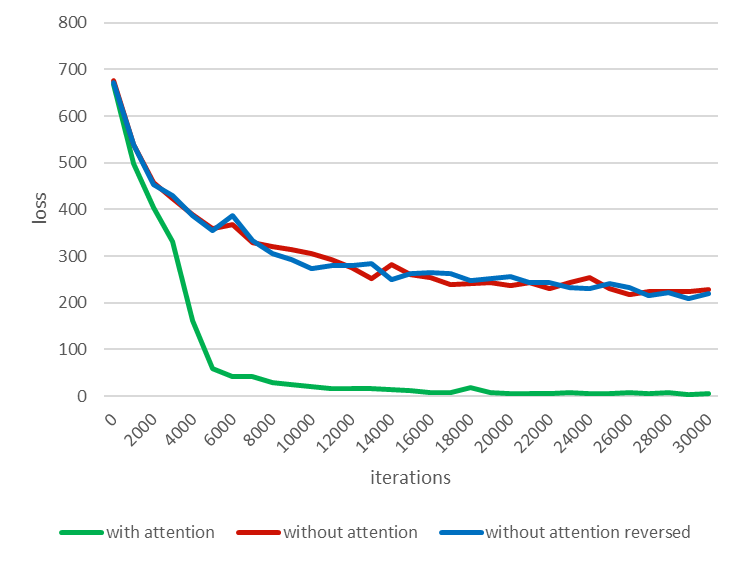
\includegraphics[width=0.9\linewidth]{attention_chart}
\caption{The training loss of models with or without an attention mechanism as a function over iterations.}
\label{attention_chart}
\end{figure}

Another interesting question is if the attention mechanism is essential for the model. After all, it increases complexity and training duration. To test this, the model was twice trained without the attention mechanism on top of the decoder, once with the same input the regular model got and once with the input reversed. The reversion of the input is a technique proposed in \cite{seq2seq}, the idea being to introduce more short-term dependencies while the average distance of the dependencies stays the same. This is not necessary for the regular model because the attention mechanism allows the model to take a peek of the encoder state many timesteps ago.

The experiment revealed the attention mechanism to be an essential part of the model because the models without the mechanism weren't able to solve the given task at all (see Table \ref{attention_mechanism_table}). These models never learned to repeat the input sequence probably because they couldn't pass all information from the encoder to the decoder in a single vector.

For the first couple of thousand iterations, all models learned roughly the same things, namely the general structure of the desired output. The models would start to begin the output sequence with \texttt{public ...(...)\{} and end it with \texttt{\}<eos>}. In between, they added mostly snippets that look like code but don't make any sense. However, after about 4,000 iterations the model with the attention mechanism learned to utilize the mechanism to its full potential and started repeating the input sequence. This resulted in rapid performance improvement. The training loss of the different configurations as a function over iterations can be seen in Figure \ref{attention_chart}.

The reversion of the input sequence helped the model to learn a little bit faster but overall it made almost no difference. The model was still not able to solve the task.

\subsection{RNN type}

\begin{figure}[p]
\centering
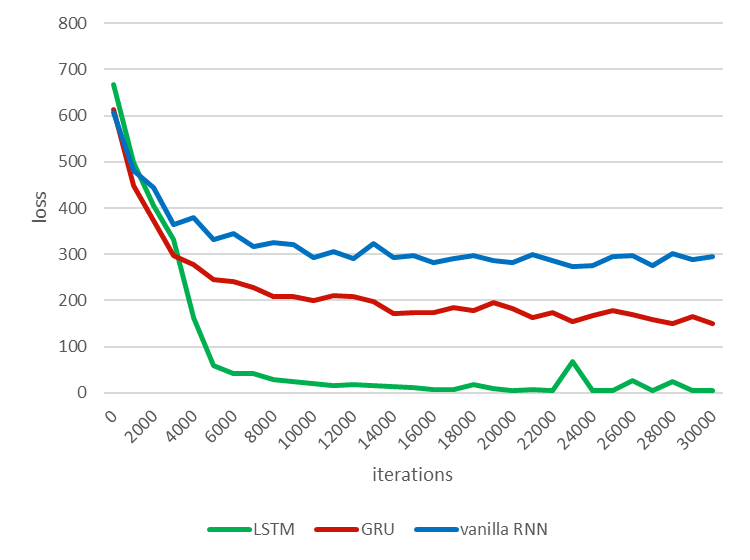
\includegraphics[width=0.9\linewidth]{cell_type_chart}
\caption{The training loss of different recurrent network types as a function over iterations.}
\label{cell_type_chart}
\end{figure}

In Subsection \ref{rnn_types} three types of RNNs were listed: vanilla RNNs, LSTMs and GRUs. To test which type works best for the given task, a model was trained for each RNN type. The training loss of the models as a function over iterations can be seen in Figure \ref{cell_type_chart}. The evaluation on the test set can be found in Table \ref{rnn_type_table}.

As could be expected the vanilla RNN performed the worst. As explained earlier, these networks have trouble with long-range dependencies and struggle with the problem of vanishing gradients. The vanilla RNN is also the simplest type and thus the one with the least amount of trainable parameters.

More surprising was the performance gap between the GRU and the LSTM, because recent research suggests that these two network types have a comparable performance \cite{lstm_vs_gru}. However similar to the models without the attention mechanism, the GRU network never fully learns to repeat the input sequence. One possible explanation for this is the fewer parameters of the GRU. An LSTM computes three gates at each timestep while also passing a memory vector to the next timestep. A GRU only has two gates and doesn't have a second vector in addition to the hidden state vector. Because the 256 units per layer are relatively few the lack of trainable parameters could prevent the GRU from learning as well as the LSTM.

\section{Error analysis}
\label{error_analysis}

In this section, the performance of the model on uncorrupted input and on each of the five corruptions is analyzed. For examples from the test set see appendix \ref{showcase}.

\subsection{Uncorrupted}

The model works reasonably well on uncorrupted input with a 70.4\% success rate. However, it is still of interest to see, what kind of errors are introduced by the network, i.e. where and why it gets confused. One mistake the model makes repeatedly is a "one-off error". Here the model would output a wrong character whose ASCII encoding is just by one off of the encoding of the correct character. For example, sometimes an asterisk whose ASCII encoding is 42 is output while the correct character would be a plus (ASCII encoding 43). If the results of the model are evaluated with a tolerance for these errors (i.e. if a character is just by one off it is not seen as an error), the accuracy of the model increases to 79.6\%. That's an almost 10\% performance increase and the model should be able to learn to avoid these mistakes with more training.

Another common error is the random switching of lines. An additional 4.8\% of the test set would have been correct if it wasn't for an incorrect line switch. This suggests that the model didn't learn to correct this corruption that well. This problem is elaborated further in Subsection \ref{switch_analysis}.

The last thing that was noticeable in the test set was that sometimes the model would get stuck in some kind of loop and output some parts or lines of the input sequence multiple times. This is something that can often be observed in the early stages of training which suggests that the model should be able to avoid these mistakes with more training.

\subsection{Missing Semicolon}

The same mistakes that were observed on uncorrupted input of course also apply to the correction of corrupted input. The correction of a missing semicolon should be the easiest error to correct and while the accuracy is already good with 71.8\% it is also worth to look at the results of an evaluation with the same "one-off tolerance" as in the evaluation of the uncorrupted results in which case the model is 81.7\% accurate. In addition to that 3.2\% of the time, an error was introduced by an incorrect line switch.

What's also interesting to see is that the output contains the correct number of semicolons in 97.0\% of the time. This means that the absence of a semicolon is detected and corrected nearly every time, there are just new mistakes that are introduced by the model into the output.

\subsection{Missing Brackets}

The main advantage of LSTMs is their ability to remember long-range dependencies which should be very useful for detecting and correcting missing brackets but the test accuracy of 51.3\% seems to contradict this assumption. However, a closer look at the results reveals that the task of inserting a missing bracket isn't that trivial. Consider the following example:

\begin{lstlisting}[style=inline]
public int addint a, int b){
  int sum = a + b;
  return sum;
}
\end{lstlisting}

Here the opening bracket between the method name and the parameters was removed. The task for the model is now to not only detect that a bracket is missing but also to find the correct spot to reinsert it which is even more difficult when there is no white space indicating the location of the missing bracket.

To see how many times the missing bracket was detected the test results were evaluated to look if the brackets in the output were balanced, meaning if every opening bracket had a closing counterpart and vice versa. The evaluation showed that the model managed to balance the brackets in 77.2\% of the time. In addition to that, the brackets were also correctly nested 76.9\% of the time which indicates that the model did learn the close open brackets very well.

\subsection{Misspelled Variable}

\begin{figure}[t]
\centering
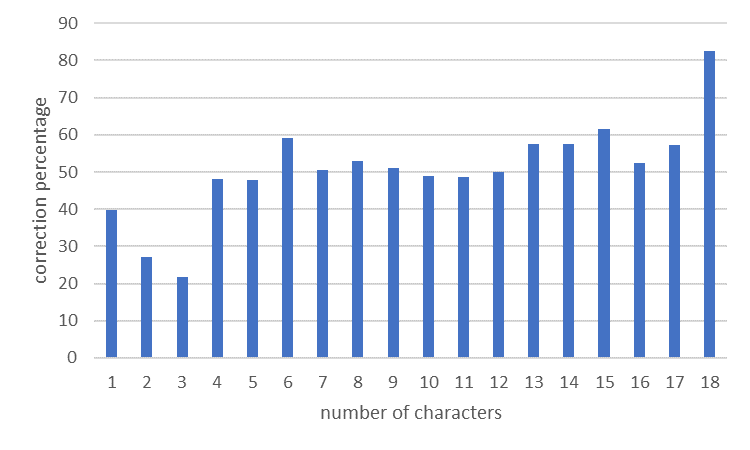
\includegraphics[width=0.9\linewidth]{variables_chart}
\caption{Correction percentages for variables of different lengths. Only lengths with more than 10 examples were considered.}
\label{variables_chart}
\end{figure}

The correction of misspelled variables was the most difficult corruption to correct for the model with an overall accuracy of 34.4\%. However when the test results are evaluated to see if the output contained the correct number of occurrences of the variable either all of them correctly spelled or all of them misspelled, the accuracy increases to 45.6\%. This includes examples where the variable was corrected but some other error was introduced to the sequence and examples where the model corrected the wrong occurrence of the variable, i.e. it corrected the variable in the declaration to conform to the introduced misspelling later in the sequence. The latter of course also result in correct code because the variable is named consistently but it is not how the model is intended to correct variables.

The accuracy of the model was also evaluated in regard to the length of the variable name. These results can be found in Figure \ref{variables_chart}. As could be expected the model struggles with variables of shorter length. This suggests that the network looks for similar patterns in the sequence to determine if a variable is misspelled and then corrects it accordingly, which is, of course, easier to do if the variable name is longer. The only big exception are one-character variables but this most likely stems from the fact that these variables have a simpler corruption pattern because there are no two characters that can be switched and the deletion of a random character doesn't serve as well so the misspelling is always an additional character that has to be removed.

\subsection{Wrong Return Type}

\begin{table}[t]
\centering
\begin{tabular}{ | l | r | }
  \hline
  Return Type & Accuracy \% \\
  \hline
  \hline
  byte(1) & 100.0 \\
  \hline
  State(15) & 86.7 \\
  \hline
  int(447) & 70.5 \\
  \hline
  void(5022) & 68.2 \\
  \hline
  String(321) & 60.8 \\
  \hline
  IFigure(284) & 44.7 \\
  \hline
  Collection(24) & 33.3 \\
  \hline
  boolean(168) & 14.3 \\
  \hline
  Double(82) & 0.0 \\
  \hline
  Session(1) & 0.0 \\
  \hline
\end{tabular}
\caption{Some return types and their correction percentages. The number in brackets indicates the number of occurrences of this type in the test set.}
\label{return_type_selection_table}
\end{table}

As discussed in Subsection \ref{corruption} it is not always possible to derive the correct return type from a method. Sometimes there is no indication of the correct type or the return type is specified as a superclass or interface of the object that is actually returned. In regard of this, the 55.1\% accuracy scored by the model is pretty good. To analyse this result further the model was evaluated to see which types it was able to correct and with which it struggled. A selection of these results can be found in Table \ref{return_type_selection_table}.

The accuracy for different data types varies greatly. There are some data types (alas not many) that the model never manages to correct. This can have different causes for example as mentioned it could be impossible to derive the correct return type or in the case of \texttt{Double} the model can also be confused by the distinction of the primitive data type \texttt{double} and its object wrapper \texttt{Double}. In the case of a \texttt{boolean} return type, there is also the additional difficulty that often no variable of type \texttt{boolean} is returned but rather a statement that resolves to a \texttt{boolean} value, e.g. \texttt{return i == 1;}.

Even though the model generally scores better on examples that occur more often, it can also be seen that this is no necessity for the model to derive the correct return type. For example, \texttt{byte} only occurs once in the test set and probably not much more in the training data and the model still managed to derive the correct return type for the method.

\subsection{Line Switch}
\label{switch_analysis}

\begin{table}[t]
\centering
\begin{tabular}{ | l | r | r | r | }
  \hline
  \(\leftrightarrow\) & VD & MI & AS \\
  \hline
  \hline
  VD & - & 53.3 & \textbf{59.3} \\
  \hline
  MI & 0.0 & - & 13.0 \\
  \hline
  AS & 0.0 & 9.8 & - \\
  \hline
\end{tabular}
\caption{The correction percentages for different line switches. The rows indicate the type of the first line and the columns the type of the second line. There are three possible types: variable declaration (VC), method invocation (MI) or assignment (AS). Only lines of different types were switched.}
\label{switch_table}
\end{table}

At first sight, the performance of the model on the switched lines corruption appears to be pretty good with 42.6\%. However, observations from the previous subsections suggest that the model still gets confused with some line switches. For this purpose, the test results were evaluated with regard to the type of the switched lines. The scores can be found in Table \ref{switch_table}.

It quickly becomes apparent that the model only really learns to correct line switches where the first line is a variable declaration. These switches mostly produce semantic errors rather than logic ones because often the declared variable is used in the other line and therefore before it was declared after the switch. For example the error in:

\begin{lstlisting}[style=inline]
public int add(int a, int b){
  sum = a + b;
  int sum;
  return sum;
}
\end{lstlisting}

\noindent is a semantic one and not a logic one. Furthermore by going through the test results, one can see that the other switches often don't produce any error at all (examples can be found in Appendix \ref{showcase}). Unfortunately, it is not possible to evaluate the percentage of introduced errors quantitatively because there would be no need to train a model on the task of logic error detection if it could already be done reliably.

Nevertheless, it is reasonable to draw the conclusion that the model gets confused by the line switches with low correction accuracy because it cannot figure out when and how they occur. This is probably the reason for the random line switches discussed in previous subsections. These low accuracy switches are also the ones that are not very likely to produce an error.

\newpage{\pagestyle{empty} \cleardoublepage}

\chapter{Conclusion}
\section{Future Work}

\newpage{\pagestyle{empty} \cleardoublepage}

\begin{appendix}
\chapter{Used Notation}
\section{Naming Conventions}

Vector and matrix variables are written in bold, vectors having lowercase names, matrices uppercase ones.

\begin{equation*}
  \mathbf{a}_t, \mathbf{B}
\end{equation*}

If no other indication of the nature of the variable is given, it is a vector resp. matrix of learnt parameters. These variables are often named \(\mathbf{W}\) for matrices and \(\mathbf{v}\) for vectors.

\bigskip

The individual elements of a vector are not written in bold and are indexed with a subscript.

\begin{equation*}
  \mathbf{a} = \begin{pmatrix} a_1 \\ ... \\ a_n \end{pmatrix}
\end{equation*}

If the vector already has a subscript, the index of the element is added as an additional subscript.

\begin{equation*}
  \mathbf{a}_i = \begin{pmatrix} a_{i1} \\ ... \\ a_{in} \end{pmatrix}
\end{equation*}

\section{Vector Operations}

For \(\mathbf{a}^\intercal = \begin{pmatrix} a_1 & ... & a_n \end{pmatrix}\) and \(\mathbf{b}^\intercal = \begin{pmatrix} b_1 & ... & b_n \end{pmatrix}\), \(\odot\) depicts the elementwise multiplication.

\begin{equation*}
  \mathbf{a} \odot \mathbf{b} = \begin{pmatrix} a_1 * b_1 \\ ... \\ a_n * b_n \end{pmatrix}
\end{equation*}

The concatenation of vectors is abbreviated as follows:

\begin{equation*}
  \begin{pmatrix} \mathbf{a} \\ \mathbf{b} \end{pmatrix} = \begin{pmatrix} a_1 \\ ... \\ a_n \\ b_1 \\ ... \\ b_n \end{pmatrix}
\end{equation*}

\chapter{Showcase}
\label{showcase}
This is a showcase

\clearpage
\pagestyle{empty}
\begin{landscape}
\begin{table}[p]
\begin{tabular}{ | m{10cm} | m{10cm} | }
  \hline
  Uncorrupted Input & Output \\
  \hline
  {\begin{lstlisting}[style=table]
  public final void enable() {
    FileConfiguration config = new FileConfiguration(NoLagg.plugin);
    config.load();
    this.enable(config);
    config.save();
  }
  \end{lstlisting}} &
  {\begin{lstlisting}[style=table]
  public final void enable() {
   FileConfiguration config = new FileConfiguration(NoLagg.plugin);
   config.load();
   this.enable(config);
   config.save();
  }
  \end{lstlisting}} \\
  \hline
  {\begin{lstlisting}[style=table]
  private Vec4 parseVec4(String s) {
   Scanner snr = new Scanner(s);
   Vec4 res = new Vec4();
   res.x = Float.parseFloat(snr.next());
   res.y = Float.parseFloat(snr.next());
   res.z = Float.parseFloat(snr.next());
   res.w = Float.parseFloat(snr.next());
   return res;
  }
  \end{lstlisting}} &
  {\begin{lstlisting}[style=table]
  private Vec4 parseVec4(String s) {
   Scanner snr = new Scanner(s);
   Vec4 res = new Vec4();
   res.x = Float.parseFloat(snr.next());
   res.y = Float.parseFloat(snr.next());
   res.$y$ = Float.parseFloat(snr.next());
   res.w = Float.parseFloat(snr.next());
   return res;
  }
  \end{lstlisting}} \\
  \hline
\end{tabular}
\caption{Example}
\label{uncorrupted_showcase_table}
\end{table}

\begin{table}[p]
\begin{tabular}{ | m{10cm} | m{10cm} | }
  \hline
  Brackets Input & Output \\
  \hline
  {\begin{lstlisting}[style=table]
  int pop(int numBits) $_$
   int i = getLeadingAsInt(numBits);
   truncate(numBits);
   return i;
  }
  \end{lstlisting}} &
  {\begin{lstlisting}[style=table]
  int pop(int numBits) ^{^
   int i = getLeadingAsInt(numBits);
   truncate(numBits);
   return i;
  }
  \end{lstlisting}} \\
  \hline
  {\begin{lstlisting}[style=table]
  protected void outlineShape(Graphics graphics, Rectangle bounds) {
   PointList pl = setupPoints$_$bounds);
   graphics.drawPolygon(pl);
   int add = graphics.getLineWidth() / 2;
   graphics.drawOval(new Rectangle(ovalX, ovalY, ovalD + add, ovalD + add));
  }
  \end{lstlisting}} &
  {\begin{lstlisting}[style=table]
  protected void outlineShape(Graphics graphics, Rectangle bounds) {
   PointList pl = setupPointsbounds$($);
   graphics.drawPolygon(pl);
   int add = graphics.getLineWidth() / 2;
   graphics.drawOval(new Rectangle(ovalX, ovalY, ovalD + add, ovalD + add));
  }
  \end{lstlisting}} \\
  \hline
\end{tabular}
\caption{Example}
\label{brackets_showcase_table}
\end{table}

\begin{table}[p]
\begin{tabular}{ | m{10cm} | m{10cm} | }
  \hline
  Semicolons Input & Output \\
  \hline
  {\begin{lstlisting}[style=table]
  @Override
  public Method run() {
   try {
    final Method mtd = clazz.getMethod("writeReplace")$_$
    mtd.setAccessible(true);
    return mtd;
   } catch (NoSuchMethodException e) {}
   return null;
  }
  \end{lstlisting}} &
  {\begin{lstlisting}[style=table]
  @Override
  public Method run() {
   try {
    final Method mtd = clazz.getMethod("writeReplace")^;^
    mtd.setAccessible(true);
    return mtd;
   } catch (NoSuchMethodException e) {}
   return null;
  }
  \end{lstlisting}} \\
  \hline
  {\begin{lstlisting}[style=table]
  public void test_hashCode() {
   ExternalIdWithDates d1a = ExternalIdWithDates.of(IDENTIFIER, VALID_FROM, VALID_TO);
   ExternalIdWithDates d1b = ExternalIdWithDates.of(IDENTIFIER, VALID_FROM, VALID_TO);
   assertEquals(d1a.hashCode(), d1b.hashCode())$_$
  }
  \end{lstlisting}} &
  {\begin{lstlisting}[style=table]
  public void test_hashCode() {
   ExternalIdWithDates d1a = ExternalIdWithDates.of(IDENTIFIER, VALID_TO);
   ExternalIdWithDates d1b = ExternalIdWithDates.of(IDENTIFIER, VALID_TO);
   assertEquals(d1a.hashCode(), d1b.hashCode());
   $assertEquals(d1a.hashCode(), d1b.hashCode());$
  }
  \end{lstlisting}} \\
  \hline
\end{tabular}
\caption{Example}
\label{semicolon_showcase_table}
\end{table}

\begin{table}[p]
\begin{tabular}{ | m{10cm} | m{10cm} | }
  \hline
  Variable Input & Output \\
  \hline
  {\begin{lstlisting}[style=table]
  private boolean validateOrder(InteractionOperand interactionOperand) {
   orderedFragments = $interactionOpernd$.getFragments();
   computeConstraints();
   return reorderFragmentsInAValidTrace();
  }
  \end{lstlisting}} &
  {\begin{lstlisting}[style=table]
  private boolean validateOrder(InteractionOperand interactionOperand) {
   orderedFragments = ^interactionOperand^.getFragments();
   computeConstraints();
   return reorderFragmentsInAValidTrace();
  }
  \end{lstlisting}} \\
  \hline
  {\begin{lstlisting}[style=table]
  @Override
  public void mouseReleased(MouseEvent e) {
   popup.setVisible(false);
   String colorText = "RGB = " + buttonColor.getRed() + ", " + buttonColor.getBreen() + ", " + buttonColor.getBlue();
   this.setText($colrText$);
   this.firePropertyChange(COLOR_CHANGE, previousColor, buttonColor);
  }
  \end{lstlisting}} &
  {\begin{lstlisting}[style=table]
  @Override
  public void mouseReleased(MouseEvent e) {
   popup.setVisible(false);
   String colorText = "RGB = " + buttonColor.getRed() + ", " + buttonColor.getBreen() + ", " + buttonColor.getBlue();
   this.setText($colrText$);
   this.firePropertyChange(COLOR_CHANGE, previousColor, buttonColor);
  }
  \end{lstlisting}} \\
  \hline
\end{tabular}
\caption{Example}
\label{variable_showcase_table}
\end{table}

\begin{table}[p]
\begin{tabular}{ | m{10cm} | m{10cm} | }
  \hline
  Return type Input & Output \\
  \hline
  {\begin{lstlisting}[style=table]
  @Override
  public $void$ toString() {
   if (eIsProxy()) return super.toString();
   StringBuffer result = new StringBuffer(super.toString());
   result.append(" (name: ");
   result.append(name);
   result.append(')');
   return result.toString();
  }
  \end{lstlisting}} &
  {\begin{lstlisting}[style=table]
  @Override
  public ^String^ toString() {
   if (eIsProxy()) return super.toString();
   StringBuffer result = new StringBuffer(super.toString());
   result.append(" (name: ");
   result.append(name);
   result.append(')');
   return result.toString();
  }
  \end{lstlisting}} \\
  \hline
  {\begin{lstlisting}[style=table]
  @Override
  public $void$ evaluate(final Double...ts) {
   Validate.isTrue(ts.length == 2);
   final double tau = ts[0];
   final double s = ts[1];
   final double t = maturity - tau;
   final double temp = vol * Math.pow(s, beta) * localVol.getVolatility(t, s);
   return -0.5 * temp * temp;
  }
  \end{lstlisting}} &
  {\begin{lstlisting}[style=table]
  @Override
  public $Validate$ evaluate(final Double...ts) {
   $>$final double tau = ts[0];
   $>$Validate.isTrue(ts.length == 2);
   final double s = ts[1];
   final double t = maturity - tau;
   final double temp = vol * Math.pow(s, beta) * localVol.getVolatility(t, s);
   return -0.5 * temp * temp;
  }
  \end{lstlisting}} \\
  \hline
\end{tabular}
\caption{Example}
\label{return_type_showcase_table}
\end{table}

\begin{table}[p]
\begin{tabular}{ | m{10cm} | m{10cm} | }
  \hline
  Switch Input & Output \\
  \hline
  {\begin{lstlisting}[style=table]
  protected void disposeElementInfo(Object element, ElementInfo info) {
   if (info instanceof ResourceSetInfo) {
    $>$resourceSetInfo.dispose();
    $>$ResourceSetInfo resourceSetInfo = (ResourceSetInfo) info;
   }
   super.disposeElementInfo(element, info);
  }
  \end{lstlisting}} &
  {\begin{lstlisting}[style=table]
  protected void disposeElementInfo(Object element, ElementInfo info) {
   if (info instanceof ResourceSetInfo) {
    ^>^ResourceSetInfo resourceSetInfo = (ResourceSetInfo) info;
    ^>^resourceSetInfo.dispose();
   }
   super.disposeElementInfo(element, info);
  }
  \end{lstlisting}} \\
  \hline
  {\begin{lstlisting}[style=table]
  private void resolveEntry(Entry < K, T > entry) {
   $>$entry.isResolved = true;
   $>$resolved.add(entry);
   resolved(entry);
  }
  \end{lstlisting}} &
  {\begin{lstlisting}[style=table]
  private void resolveEntry(Entry < K, T > entry) {
   $>$entry.isResolved = true;
   $>$resolved.add(entry);
   resolved(entry);
  }
  \end{lstlisting}} \\
  \hline
\end{tabular}
\caption{Example}
\label{switch_showcase_table}
\end{table}
\end{landscape}
\clearpage

\newpage{\pagestyle{empty} \cleardoublepage}
\end{appendix}

\addcontentsline{toc}{chapter}{\numberline{}List of Tables}
\listoftables

\addcontentsline{toc}{chapter}{\numberline{}List of Figures}
\listoffigures

\addcontentsline{toc}{chapter}{\numberline{}Bibliography}
\bibliographystyle{plaindin}
\nocite{*}
\bibliography{bibliography}

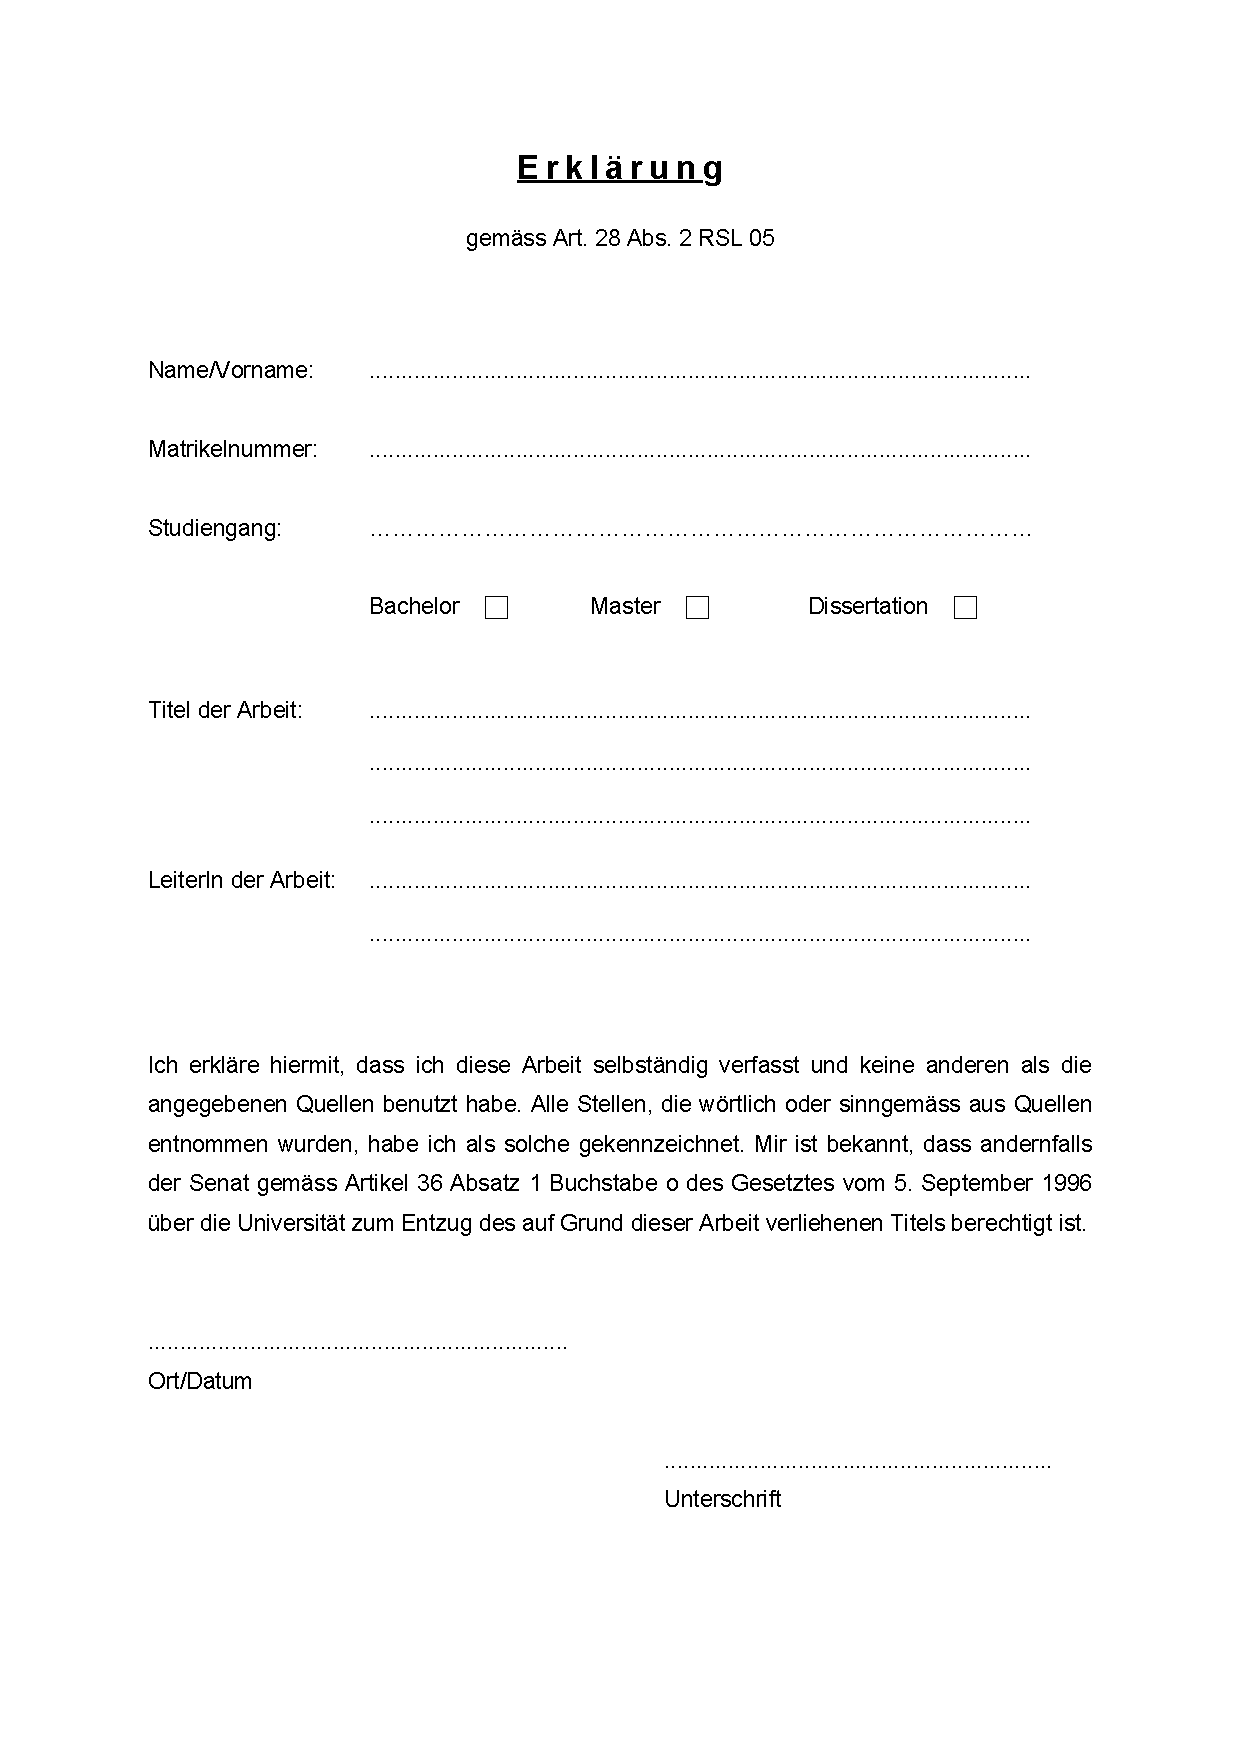
\includepdf{Erklaerung.pdf}

\end{document}
